% !TEX encoding = UTF-8 Unicode

\Chapter{Implementáció C++ és OpenCV segítségével}
\label{chap:implement}

\Section{OpenCV bemutatása}

Az OpenCV (Open Source Computer Vision Library) egy nyílt forráskódú számítógépes látás és gépi tanulási szoftverkönyvtár \cite{opencv}. Az OpenCV-t azért hozták létre, hogy közös infrastruktúrát biztosítson a számítógépes megjelenítési alkalmazások számára, és felgyorsítsa a gépi érzékelés használatát a kereskedelmi termékekben. BSD licenc alatt került kiadásra, ezért ingyenes mind tudományos, mind kereskedelmi célokra. C++, Python és Java interfészekkel rendelkezik, és támogatja a Windows, Linux, Mac OS, iOS és Android rendszereket. Az OpenCV-et a számítási hatékonyságra tervezték, és nagy hangsúlyt fektetett a valós idejű alkalmazásokra. Az optimalizált C/C++-ban írt, a könyvtár kihasználhatja a többmagos feldolgozást is. Az OpenCL használatával kihasználhatja az alapul szolgáló heterogén számítási platform hardveres gyorsítását.

A könyvtár több mint 2500 optimalizált algoritmussal rendelkezik, amely magába foglalja mind a klasszikus, mind a legmodernebb számítógépes látásmódot és a gépi tanulási algoritmusokat. Ezek az algoritmusok felismerhetik az arcokat, felismerhetik az objektumokat, osztályozhatják az emberi cselekvéseket a videókban, nyomon követhetik a mozgásokat, követhetik a mozgó objektumokat, eltávolíthatja a vörös szemeket a vakuval készített képekből, követheti a szemmozgásokat, felismerheti a tájat stb. 

% https://opencv.org

\Section{Beépített művészi jellegű OpenCV-s szűrők}

Az OpenCV könyvtár rendelkezik saját bepített, nem fotorealisztikus szűrőkkel, amelyeknél csak a bemeneti képet, valamint néhány paramétert kell megadnunk a függvénynek és ő elkészíti nekünk a filterezett képet. Négy ilyen beépített függvény található az OpenCV-ben, Edge Preserving filter, Detail Enhancing filter, Pencil sketch filter és a Stylization filter. Ezek C++ implementációját szeretném bemutatni.

\SubSection{Edge Preserving filter}

Az első ilyen szűrő az \textit{Edge Preversing filter}, ami az éleket megörzi de a hátteret elmossa. 
Ennek a paraméterezése az alábbi
\begin{cpp}
edgePreservingFilter(Mat src, Mat dst, int flags=1, 
			float sigma_s=60, float sigma_r=0.4f);
\end{cpp}
ahol,
\begin{itemize}
    \item \texttt{src}: a bemeneti kép, amit szertnénk átalakítani,
    \item \texttt{dst}: a filterrel ellátot kép,
    \item \texttt{flags}: maga az él kiemelő filter melynek két paramétere lehet, \texttt{RECURS\_FILTER} (rekurív szűrő) aminek az értéke 1 vagy \texttt{NORMCONV\_FILTER} (normalizált konvolúció) aminek az értéke 2.  A futási sebességtől függ melyik paramétert alkalmazzuk, ha gyorsabb sebességet akarounk elérni akkor a rekurzív filtert alkamazzuk, ha viszont nem számít a sebesség akkor a  normalizált konvolúciót mert az szebben kiemeli az éleket.
    \item \texttt{sigma\_s}: egy skála 0 és 200 között, \texttt{Sigma\_spatial} a simítás mértékét határozzuk meg,
    \item \texttt{sigma\_r}: egy skála 0 és 1 között, \texttt{Sigma\_range} szabályozza, hogy a szomszédságon belül a különböző színek milyen mértékben átlagolódjanak.
\end{itemize}

\begin{figure}[ht]
\centering
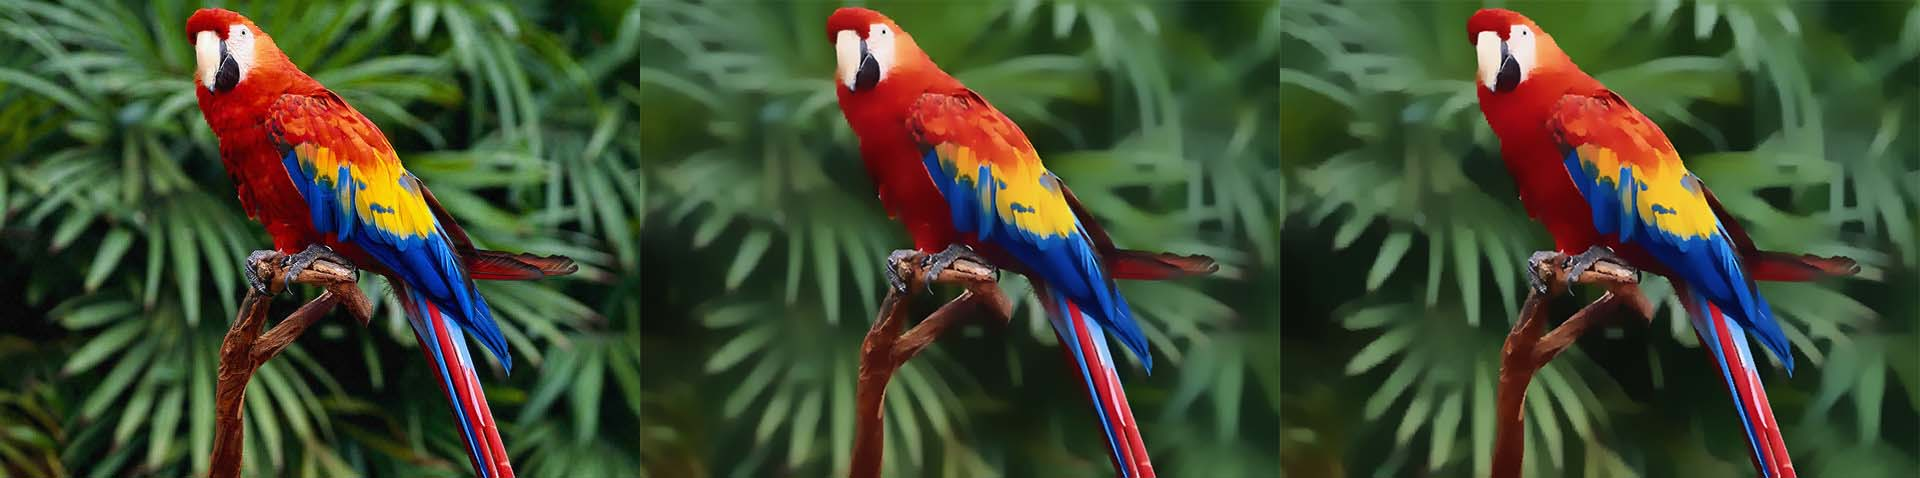
\epsfig{file=kepek/edgePreservingFilter.jpg,scale=0.45}
\caption{Eredeti kép, Rekurzív filter, Normalizált konvolúció} 
\label{fig:edgePreservingFilter}
\end{figure}

\SubSection{Detail Enhancing filter}

A második ilyen szűrő a \textit{Detail Enhancing filter}, ami a képet élesebbé teszi.
\begin{cpp}
detailEnhance(Mat src, Mat dst, float sigma_s=10, float sigma_r=0.15f);
\end{cpp}
A paraméterek megegyeznek az Edge Preserving filter paramétereivel. 

\begin{figure}[ht]
\centering
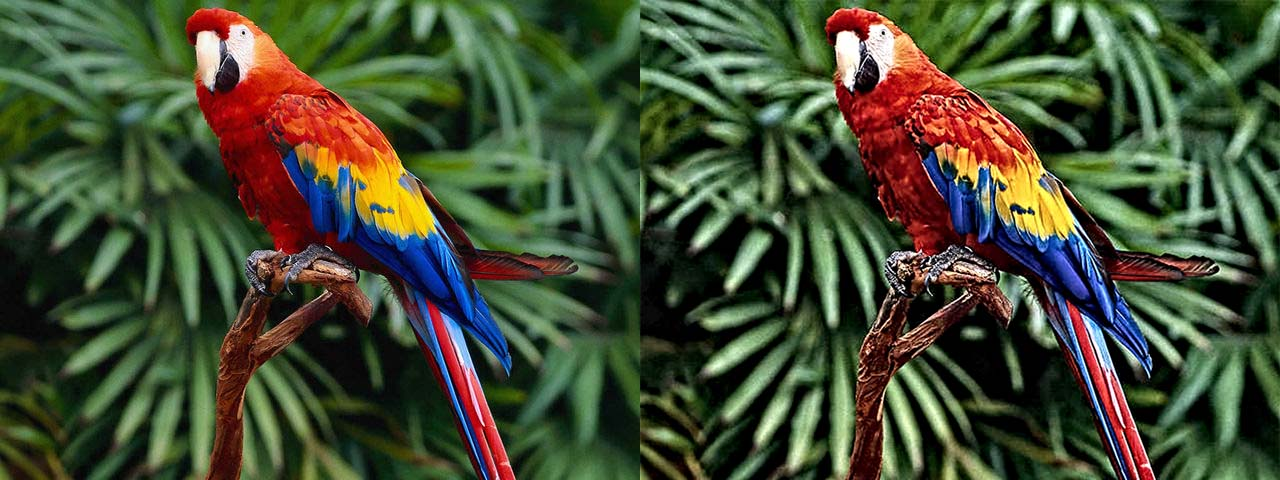
\epsfig{file=kepek/detailEnhance.jpg,scale=0.65}
\caption{Eredeti kép, Detail Enhancing filter eredménye} 
\label{fig:detailEnhance}
\end{figure}

\SubSection{Pencil sketch filter}

Ez a szűrő ceruza rajzot eredményez, két féle képet eredményez egy színes képet és egy szürkeárnyalatosat.
\begin{cpp}
pencilSketch(Mat src, Mat dst_gray, Mat dst_color, float sigma_s=60, 
		float sigma_r=0.07f, float shade_factor=0.02f);
\end{cpp}
A paraméterek megegyeznek az Edge Preserving szűrőével, de bővül az alábbi paraméterrel:
\begin{itemize}
    \item \texttt{shade\_factor}: ami egy 0 és 0,1 közötti érték, a kimeneti képintenzitás skálázása. Minél magasabb az érték, annál fényesebb az eredmény.
\end{itemize}

\begin{figure}[ht]
\centering
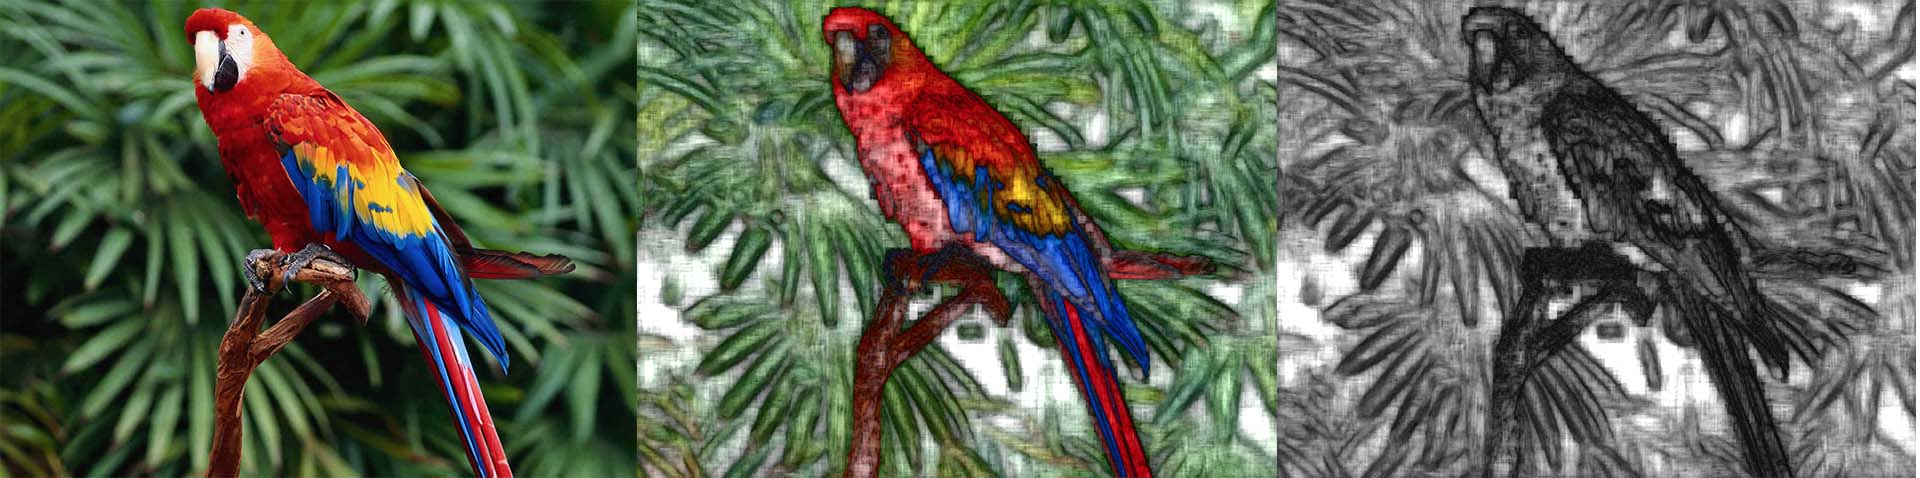
\epsfig{file=kepek/pencil_sketch_color_grey.jpg,scale=0.45}
\caption{Eredeti kép, Pencil sketch filter színes, Pencil sketch filter szűrkeárnyalatos} 
\label{fig:pencil_sketch_color_grey}
\end{figure}

\SubSection{Stylization filter}

A Stylization filter olyan kimeneti képet eredményez, aminek olyan hatása van mint ha vízfestékkel készítették volna.
\begin{cpp}
stylization(Mat src, Mat dst, float sigma_s=60, float sigma_r=0.45f);
\end{cpp}
A paraméterek megegyeznek az Edge Preserving filter paramétereivel. 

\begin{figure}[ht]
\centering
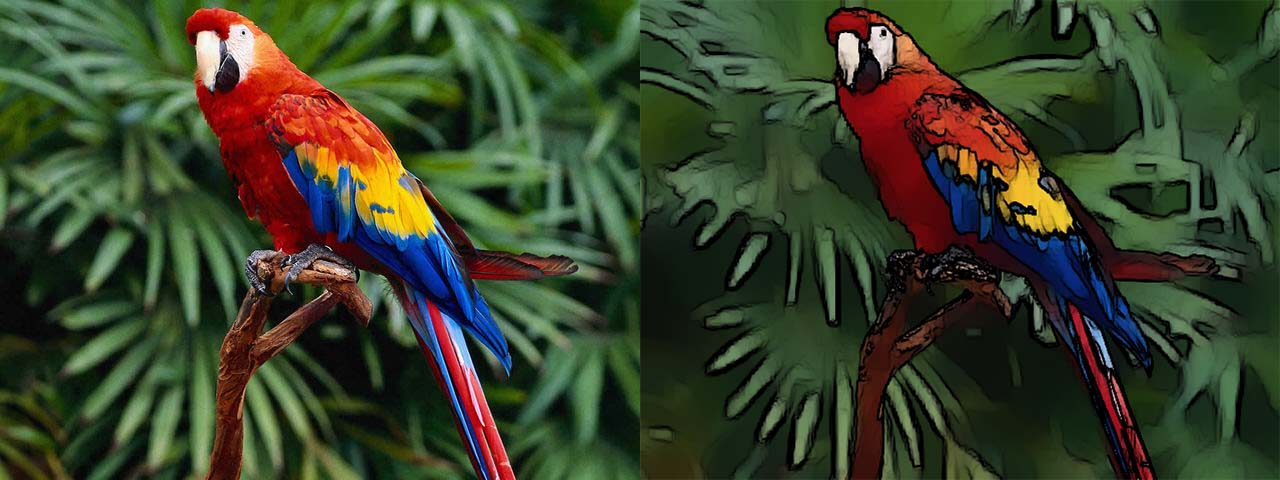
\epsfig{file=kepek/stylization.jpg,scale=0.65}
\caption{Eredeti kép, Stylization filter eredménye} 
\label{fig:stylization}
\end{figure}

%https://www.learnopencv.com/non-photorealistic-rendering-using-opencv-python-c/

\Section{Saját szűrők implementációja OpenCV és C++-al}

% TODO: Chapter reference!

Ebben a fejezetben szeretném bemutatni a saját szűrőknek a C++ implementációját és a paramétereket amiket használtam hozzájuk. Itt képekkel nem fogok illusztrálni, mert azok a \textbf{4. fejezetben} megtalálhatóak.

Elsőként bemutatnám a kép betöltésének implementációját, amit minden szűrőn használtam.
\begin{cpp}
Mat img = imread("image.jpg"); // bemeneti kep
Mat dst; // kimeneti kep
// Ha valami nem stimmel a kep betoltesnel
if (img.empty()) {
    cout << "Error loading the image" << endl;
    return -1;
}
\end{cpp} 
Ablak létrehozása :
\begin{cpp}
namedWindow("Original image", 1);
namedWindow("Image with filter", 1);
\end{cpp}
Ezután következik az a rész, amit a következő alfejezetekben fogok részletezni, hogy tulajdon képpen milyen lépésekből épül fel a filter. Ezek után a kép megjelenítése:
\begin{cpp}
imshow("Original imagel",img );
imshow("Image with filter", dst);
\end{cpp} 
\newpage
\noindentÉs végezetül a waitKey funkció következik, amely a megadott milliszekundumban megjeleníti a képet. Mivel itt nem mozgó képről beszélünk igy az értéke 0.
\begin{cpp}
waitKey(0);
\end{cpp}
\SubSection{Cartoon-style filter}
Gauss piramisban lefelé lépünk kettőt.
\begin{cpp}
for (int i = 0; i < 2; i++) {
    pyrDown(img, img);
}
\end{cpp}
ahol,
\begin{itemize}
    \item \texttt{img}: a bemeneti színes kép,
    \item \texttt{img}: a kimeneti kicsinyített színes kép.
\end{itemize}
Egymás után hétszer hajtjuk végre a kétoldalú szűrőt.
\begin{cpp}
Mat img_res;
int d = 9;
double sigmaColor = 9.0;
double sigmaSpace = 7.0;
for (int i = 0; i < 7; i++) {
    bilateralFilter(img, img_res, d, sigmaColor, sigmaSpace);
}
\end{cpp}
ahol,
\begin{itemize}
    \item \texttt{img}: a bemeneti színes kép,
    \item \texttt{img\_res}: a kimeneti kép kétoldalú szűrővel,
    \item \texttt{d}: a szűrés során használt minden egyes pixel szomszédság átmérője. Ha nem pozitív, akkor kiszámítható a sigmaSpace-ből,
    \item \texttt{sigmaColor}: szűri a szigmát a színtérben,
    \item \texttt{sigmaSpace}: szűri a szigmát a koordinátatérben.
\end{itemize}
Gauss piramisban felfelé lépünk kettőt, hogy visszanyerjük az eredeti kép méretet.
\begin{cpp}
for (int i = 0; i < 2; i++) {
    pyrUp(img_res, img_res);
}
\end{cpp}
ahol,
\begin{itemize}
    \item \texttt{img\_res}: a bemeneti kép kétoldalú szűrővel,
    \item \texttt{img\_res}: a kimeneti nagyított színes kép.
\end{itemize}
Egy képet a
\begin{cpp}
cvtColor(img, srcGray, CV_BGR2GRAY);
\end{cpp}
utasítással konvertálhatunk szürkeárnyalatossá, amelyben
\begin{itemize}
    \item \texttt{img}: a bemeneti színes kép,
    \item \texttt{srcGray}: a kimeneti szürkeárnyalatos kép,
    \item \texttt{CV\_BGR2GRAY}: színes kép szürkeárnyalatosra alakítására használatos paraméter.
\end{itemize}
A következő lépésben a medián szűrőt implementáltam az
\begin{cpp}
int kernel_size = 7;
medianBlur(srcGray, median, kernel_size);
\end{cpp}
formában, ahol
\begin{itemize}
    \item \texttt{srcGray}: a bemeneti szürkeárnyalatos kép,
    \item \texttt{median}: a kimeneti medián szűrővel ellátott kép,
    \item \texttt{kernel\_size}: a kernel mérete, itt ebben az esetben egy $7 \times 7$-es mátrix. Ami már nem csak a zaj kiszűrését eredményezi, hanem már cartoon jellegűre mossa a képet.
Adaptív küszöbölés implementációja.
\end{itemize}
\begin{cpp}
Mat img_edge;
double maxValue = 225;
int blockSize = 9;
double C = 2; 
adaptiveThreshold(median,img_edge, maxValue, ADAPTIVE_THRESH_MEAN_C,
		THRESH_BINARY, blockSize, C); 
\end{cpp}
ahol,
\begin{itemize}
    \item \texttt{median}: a bemeneti medián szűrővel ellátott kép,
    \item \texttt{img\_edge}: a kimeneti éldetektálás eredménye,
    \item \texttt{maxValue}: nem zérus érték hozzárendelve azokhoz a képpontokhoz, amelyekhez a feltétel teljesül.
    \item \texttt{ADAPTIVE\_THRESH\_MEAN\_C}: adaptiv küszöbölés algoritmus,
    \item \texttt{THRESH\_BINARY}: a küszöbérték típusának \texttt{THRESH\_BINARY} vagy \texttt{THRESH\_BINARY\_INV} értékűnek kell lennie,
    \item \texttt{blockSize}: a pixel szomszédságának mérete, amelyet a pixel küszöbértékének kiszámítására használnak,
    \item \texttt{C}: a konstanst az átlagból vagy a súlyozott átlagból kell levonni, normális esetben pozitív, de lehet nulla vagy negatív is.
\end{itemize}
A maszk színesre konvertálása.
\begin{cpp}
cvtColor(img_edge, img_edge, CV_GRAY2RGB);
\end{cpp}
ahol,
\begin{itemize}
    \item \texttt{img\_edge}: a bemeneti szürkeárnyalatos kép,
    \item \texttt{img\_edge}: a kimeneti színes kép,
    \item \texttt{CV\_GRAY2RGB}: szürkeárnyalatos kép színesre alakítására használatos paraméter.
\end{itemize}
Az elmosott képet és a maszkot 
\begin{cpp}
Mat img_cartoon;
bitwise_and(img_res, img_edge, img_cartoon);
\end{cpp}
programsorokkal egyesíthetjük, ahol
\begin{itemize}
    \item \texttt{img\_res}: a bemeneti elmosott kép,
    \item \texttt{img\_edge}: a bemeneti élmaszk,
    \item \texttt{img\_cartoon}: kimeneti Cartoon-style filterezett kép.
\end{itemize}

\SubSection{Pencil sketch filter}

Első lépésként átkonvertáltam a képet színesről szűrkeárnyalatossá majd egy medián szűrést hajtottam végre. Ezt az előző szűrőnél már bemutattam így itt nem részletezném, annyiban változik a paraméterezése, hogy a kernel mérete itt egy $3 \times 3$-as mátrix.
A következő lépésben egy Gauss simítást implementáltam. 
\begin{cpp}
Mat gauss;
Size ksize = Size(21, 21);
double sigmaX = 0;
double sigmaY = 0;
GaussianBlur(median, gauss, ksize, sigmaX, sigmaY);
\end{cpp}
ahol,
\begin{itemize}
    \item \texttt{median}: a bemeneti medián szűrővel ellátott kép,
    \item \texttt{img\_blur}: a kimeneti Gauss szűrés eredménye,
    \item \texttt{ksize}: a kernel mérete, itt ebben az esetben egy $21 \times 21$-es mátrix,
    \item \texttt{sigmaX}: a Gauss kernel standard elterese $x$ iranyba,
    \item \texttt{sigmaY}: a Gauss kernel standard elterese $y$ iranyba.
\end{itemize}
A medián és Gauss szűrő elosztása egymással.
\begin{cpp}
Mat img_blend;
double scale_d = 245;
divide(median, gauss, img_blend, scale_d);   
\end{cpp}
ahol,
\begin{itemize}
    \item \texttt{median}: a bemeneti medián szűrővel ellátott kép,
    \item \texttt{img\_blur}: a bemeneti Gauss szűrővel ellátott kép,
    \item \texttt{img\_blend}: a kimeneti kép a szűrők elosztásának eredménye,
    \item \texttt{scale\_d}: a skalár tényező.
\end{itemize}
Kontraszt széthúzás.
\begin{cpp}
double alpha=0; 
double beta=255;
normalize(img_blend, img_blend, alpha, beta, CV_MINMAX);
\end{cpp}
ahol,
\begin{itemize}
    \item \texttt{img\_blend}: a két szűrő elosztásával kapott kép,
    \item \texttt{img\_blend}: a kimeneti kontraszt széthúzással kapott kép,
    \item \texttt{alpha}: normál érték a normálértékhez viszonyítva vagy az alsó tartomány határértéke esetén,
    \item \texttt{beta}: első tartományhatár a tartomány normalizálása esetén,
    \item \texttt{CV\_MINMAX}: választható maszk művelet.
\end{itemize}
A szürkeárnyalatos vászon összeszorzása a kontraszt széthúzott képpel.
\begin{cpp}
double scale_m = 1.0 / 256;
multiply(img_blend, canvas, img_blend, scale_m);
\end{cpp}
ahol,
\begin{itemize}
    \item \texttt{img\_blend}: a bemeneti kontraszt széthúzással ellátott kép,
    \item \texttt{canvas}: a bemenet vászon képe,
    \item \texttt{img\_blend}: a kimeneti összeszorzott kép,
    \item \texttt{scale\_m}: választható skálafaktor.
\end{itemize}

\SubSection{Cartoon filter}

Első lépésként itt mint az előző filtereknél, átkonvertáltam a képet színesről szűrkeárnyalatossá majd egy medián szűrést hajtottam végre, ahol a kernel mérete $7 \times 7$-es matrix.
Ezt egy Laplace éldetektálás követte.
\begin{cpp}
int kernel_size = 5;  
Laplacian(median, edges, CV_8U, kernel_size);
\end{cpp}
ahol,
\begin{itemize}
    \item \texttt{median}: a bemeneti median szűrővel ellátott kép,
    \item \texttt{edges}: az élekdetektálás eredménye,
    \item \texttt{CV\_8U}: unsigned 8bit/pixel, azaz egy pixel $[0, 255]$ egész értékű tartományban lehet,
    \item \texttt{kernel\_size}: a kernel mérete, itt ebben az esetben egy $5 x 5$-ös mátrix. Azt mutatja meg mekkora legyen a maszkon az él mérete.
\end{itemize}
Végezetül a küszöbölés következett.
\begin{cpp}
double thresh = 90;
double maxval = 255;
threshold(edges, mask, thresh, maxval, THRESH_BINARY_INV);
\end{cpp}
ahol,
\begin{itemize}
    \item \texttt{edges}: a bemeneti kép az élekdetektálás eredménye,
    \item \texttt{mask}: a küszöbölés eredménye,
    \item \texttt{thresh}: küszöbérték,
    \item \texttt{maxval}: a \texttt{THRESH\_BINARY} és a \texttt{THRESH\_BINARY\_INV} küszöbérték típusokhoz használható maximális érték,
    \item \texttt{THRESH\_BINARY\_INV}:
$$
mask(x, y) = \left\{
\begin{array}{ll}
0, & \mbox{ ha edge$(x, y)$ > thresh,}\\
maxval, & \mbox{ különben}
\end{array}
\right.
$$
\end{itemize}

\SubSection{Aquarelle-stlye filter}

Ez a filter két egyszerű lépésből áll az első az egy átlagoló szűrő.
\begin{cpp}
Size ksize = Size(3, 3);
blur(img, avg, ksize);
\end{cpp}
ahol,
\begin{itemize}
    \item \texttt{img}: a bemeneti színes kép,
    \item \texttt{avg}: a kimeneti elmosott kép,
    \item \texttt{ksize}: a kernel mérete, itt ebben az esetben egy $3 \times 3$-as mátrix.
\end{itemize}
Mean shift szegmentáció.
\begin{cpp}
Mat img_shifted;
double sp = 15;
double sr = 50;
pyrMeanShiftFiltering(avg, img_shifted, sp, sr);
\end{cpp}
ahol,
\begin{itemize}
    \item \texttt{avg}: a bemeneti átlagolással elmosott színes kép,
    \item \texttt{img\_shifted}: a kimeneti mean shift szegmentálással előállított kép,
    \item \texttt{sp}: a térbeli ablak sugara,
    \item \texttt{sr}: a színablak sugara.
\end{itemize}

%4-6 oldal


% Technikai jelleg rész
